\chapter{Weak Interaction}
    \section{Fermi Interaction / Fermi Theory of Beta Decay}
        \subsection{Overview}
            \indent Early 1900s measured energy spectrum in nuclear Beta decay - expected a discrete spectrum, instead observed continuous spectrum with a clear endpoint. This prompted Pauli in 1930 to postulate the neutrino. 1931 Fermi formulated the contact formalism of beta decay.
             Proposed by Enrico Fermi in 1933. Four fermions directly interact at a singular vertex (contact interaction). First paper was originally rejected by Nature. Serves as an accurate low energy decription of weak charged current. 
        
        
            \begin{figure}[H]
                \centering
                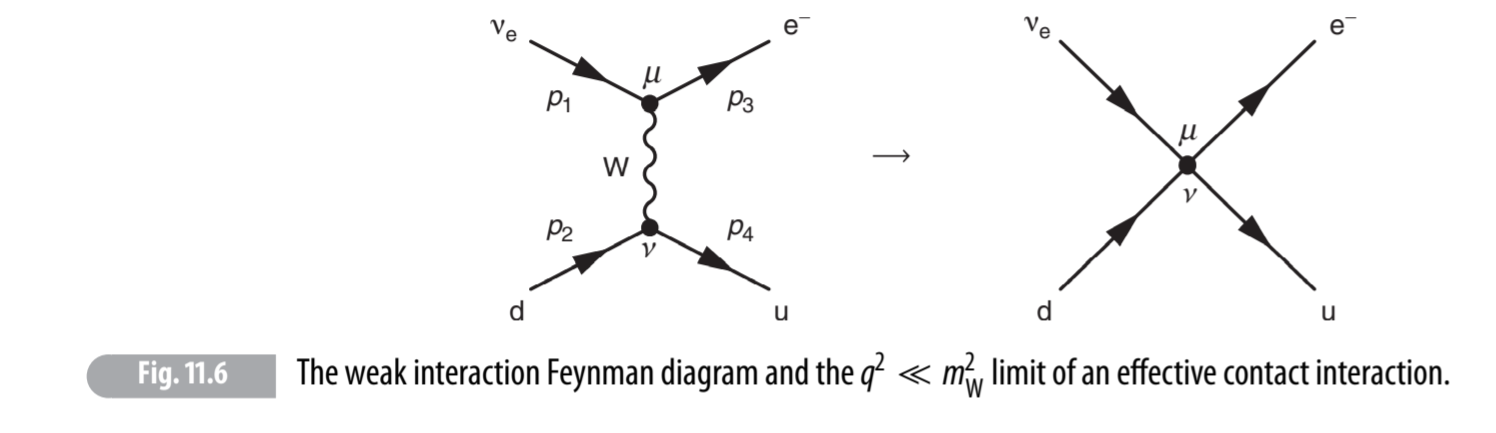
\includegraphics[width=11cm]{NuclearPhysics/modules/weak-force/pics/contact-interaction.PNG}
            \caption{Caption}
            \end{figure}
            
            
            
            \section{Beta Decays}
            beta decay:\\
            $n \longrightarrow p + e^- + \Bar{\nu}_e$ aka:\\
            $d \longrightarrow uu + e^- + \Bar{\nu}_e$\\
            beta+ decay aka positron emission\\
            $p \longrightarrow n + e^+ + \nu_e$ aka:\\
            $u \longrightarrow d + e^+ + \nu_e$ aka:\\
            electron capture aka inverse beta decay:\\
            $p + e^- \longrightarrow n + \nu_e$\\
            positron capture
            $n + e^+ \longrightarrow p + \Bar{\nu}_e$\\
            double beta decay
            neutrinoless double beta decay
            
            
        
        \section{Transitions}
            Describe nuclear beta decay by changes in angular momentum or spin. 
            \subsection{Fermi Transition}
                Spins of emitted particles are antiparallel, copuling to S=0, so the angular momentum of the initial and final angular momentum states are unchanged ($\Delta J = 0$). E.g. no change in the total angular momentum of the nucleus. 
            \subsection{Gamow-Teller Transitions}
                Spins of the emitteded electron (positron) and antineutrino (neutrino) couple to total spin S=1, leading to angular momentum change $\Delta J = 0, \pm1$ between the initial and final angular momentum states of the nucleus.
                
                Gamow-Teller interactions are needed to describe parity violation, modifies matrix elements to include vector and axial-vector couplings of fermions. 
                
            \subsection{Forbidden Decays}
                Fermi decays are referred to as the superallowed decays, while Gamow-teller are "allowed" decays. Forbidden decays are those which are substantially more improbabe, due to parity violation, and as a result have long decay times. 
                
            \begin{figure}[H]
                \centering
                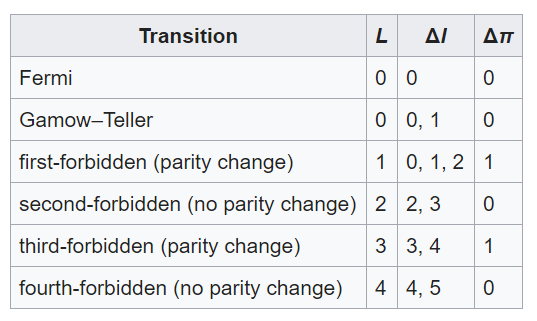
\includegraphics[width=11cm]{NuclearPhysics/modules/weak-force/pics/forbidden.PNG}
            \caption{Caption}
            \end{figure}
            
            
                Note in the above, S = 0 for Fermi, and S=1 for Gamow-Teller. 
        
                From Fermi's Golden Rule, we have the expression for the transition rate as:\\
                W = prefactors x (Matrix)$^2$ x (phase space) = 1/lifetime \\
                \newline
                
        
        \section{Relation between Fermi constant and weak constant}
            \indent $G_F$ is the Fermi coupling constant
        
        Fermi-theory fails at high energy, as the cross section grows as $G_F^2E^2$, so breaks around 100 GeV. 
        
        
        \section{Geiger-Nuttall Law}
            \indent Relation between the decay constant of an isotope with the energy of the alpha particle released in the decay. The idea is that the shorter the isotopes lifetime, the higher the alpha particle's energy is. The relation is:
            
            \begin{equation}
                \log(\ln(2)/\tau) = -a_1\frac{Z}{\sqrt{E}} + a_2
            \end{equation}
            \myequations{Geiger-Nuttall Law}
            
    \section{Scalar Vector Pseudoscalar Pseudovector Breakdown}
        \indent Scalar - number, Temperature\\
        \indent Vector - vector, momentum\\
        \indent Pseudovector - cross product of two vectors - angular momentum [N.B. - also called axial vector]\\
        \indent Pseudoscalar - product of vector and pseduovector - helicity \\
        
            
    
    \section{Wu Experiment}
        \indent Parity is the symmetry under spatial inversion through the origin, i.e. x $\longrightarrow$ -x. Spin half particle fermions have positive intrinsic parity, their antiparticles have negative intrinsic parity, Vector bosons all have negative intrinsic parity. 
        
        In 1957 C.S. Wu et. al. studied the nuclear beta decay of polarized cobalt-60:
        
        \begin{equation}
            60Co \longrightarrow 60Ni* + e^- + \Bar{\nu}_e
        \end{equation}
        
        The Cobalt-60 nuclei (spin 5/2, decays to spin 3/2, emitting away 1 unit of angular momentum), which has a permanent nuclear magnetic moment, were aligned in a strong B field. The beta-decay electrons were detected at different polar angles with respect to the magnetic field axis. If parity were conserved, the rate of electrons in one direction would be identical to the rate in the opposite direction. Instead, it was observed that more electrons were emitted int he hemisphere opposite to the applied magnetic field than in the direction of the applied field, thus proving parity violation. Below illustrates this, take the first arrow as momentum vector, and second arrow as spin vector.\\
        \newline
        Either the electron can be right handed and the anti-neutrino lefthanded:\\
       $\uparrow \longrightarrow e- \uparrow \uparrow + \Bar{\nu}_e \downarrow \uparrow$ --- not observed!!\\
       \newline
       Or the anti-neutrino can be right handed and the electron lefthanded:\\
       $\uparrow \longrightarrow \Bar{\nu}_e  \uparrow \uparrow + e^- \downarrow \uparrow$ --- observed \\
       \newline
       The way this pans out experimentally is that electrons will be detected only in the hemisphere opposite of the direction of initial spin, i.e. in the "down" direction here. 
        
        
    \section{V-A structure of Weak Interaction}
        \indent Particle interactions are expressed in the form of currents, but only Lorentz invariant combinations of particle interactions are allowed:
        
            \begin{figure}[H]
                \centering
                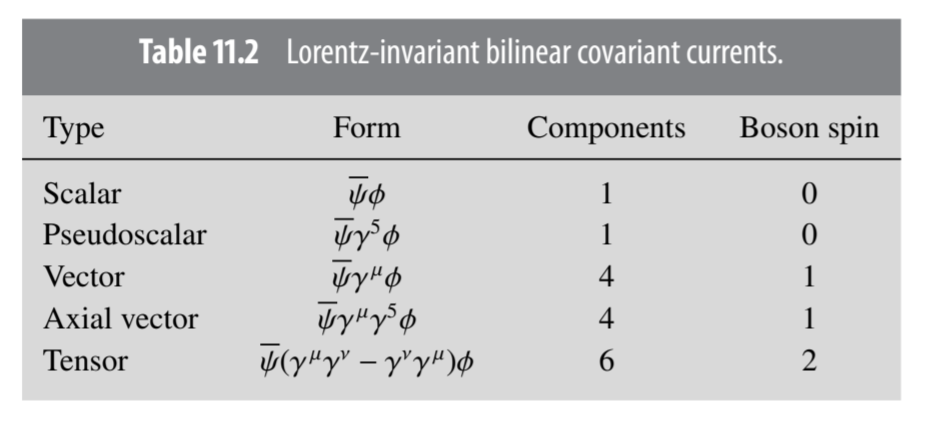
\includegraphics[width=11cm]{NuclearPhysics/modules/weak-force/pics/bilinears.PNG}
            \caption{Caption}
            \end{figure}
            
        
        QED and QCD have vector intreactions, but from considerations of parity violation, the weak force must be given by a vector minus axial vector interaction, with a vertex factor of:
        
            \begin{figure}[H]
                \centering
                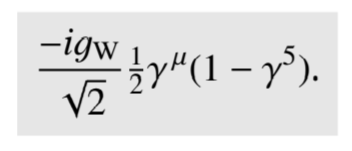
\includegraphics[width=11cm]{NuclearPhysics/modules/weak-force/pics/weak-vertex.PNG}
            \caption{Caption}
            \end{figure}
            
        
        This is obtained by considering the most general form possible, and then pairing down based off of pairity considerations, and is discussed deeply in Thomson 11.3. The important thing is that the V-A structure explicitly projects out left-handed chiral particle and right handed chiral antiparticle states.  
        
        \textbf{Experimentally}, the V-A nature is established as a fact as if the interaction were scalar or pseudoscalar, the ratio of pion to electrons vs pion to muons would be 5.5, in inexcorable contrast to experimental observations of almost all muons. The TWIST experiment observed the decays of 10 billion polarized muons, which indicate that the charged-current weak interaction is described entirely by a V-A vertex factor.\\
        
        This structure is what forces parity violation, as a LH particle that undergoes parity inversion will have its momentum flipped but spin not flipped, e.g. its helicity will flip, and it will become a RH particle, which does not interact under the weak force. 
        
    \section{Helicity in Pion Decay}
        As an applicaiton of the V-A structure, examine charge pion decay. The dominant decay modes are charged pion to muon and muon antineutrino, or to electron and electron antineutrino. Naively, due to phase space arguements, we would expect the decay to electrons to dominate by a large factor. Instead the opposite is observed. This is due to "heliciity suppresion". Specifically, the pion is spin 0, so the lepton and lepton neutrino must be emitted with oppsite spin. Since they are going in opposite directions and have opposite spin, they must be either both LH states or both RH helicity states. Since the weak force only couples to LH particle and RH anti particle chirality states, and neutrinos are essentially massless, we need to be able to boost in the lepton frame to convert from a RH particle helicity state to a LH particle state. It is much easier to boost for the 200x more massive muon, so it has more actual phase space avaliable to it. E.G. the antineutrino is always produced in a RH helicity state, so the charge lepton is also produced in a RH helicity state. The electrons are moving with $\beta = 0.99997$ while the muon is $\beta = 0.27$. For the full calculation see Thomson 11.6, but the result is that the decay rate is suppressed as approximately $m_e^2/m_{\mu}^2$, or exactly as:
        
            \begin{figure}[H]
                \centering
                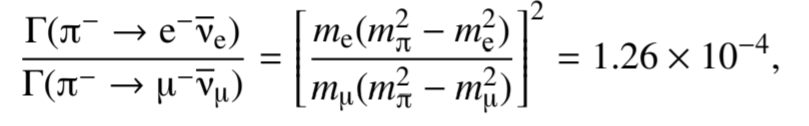
\includegraphics[width=11cm]{NuclearPhysics/modules/weak-force/pics/muon-ele-supp.PNG}
            \caption{Caption}
            \end{figure}
            
        
        
    \section{Modern Theory}
        Parity violation and renormalization suggested a reformulation of the theory. 
        Moderated by two gauge bosons:
               
               
               
            \begin{table}[H]
                \centering
                    \begin{tabular}{lllllll}
                        Boson   &   Charge    &   Mass    &   Width     &   Hadronic \%     &   Leptonic \%     &   Invisible \% \\
                        W       &  $\pm1$ &     80.4 GeV  &  2.1 GeV     &  68       &      30      &   $\sim$0      \\
                        Z       &   0 &         91.2 GeV    &   2.5 GeV    &    70     &     10  &      20 \\
                    \end{tabular}
            \end{table}
            
            Note that parity is not defied for the W or Z because they are not eigenvalues of the parity operator. The weak interaction is Vector minus Axial (V-A, equivalent to left-handed) which is not an eigenstate, this is why parity is violated in weak interactions. 
            
            The weak interaction acts only on left-handed particles and right-handed anti-particles. 
            
            The W boson differs from the photon in that it is massive, and have a longitudinal polarization state, giving the propigator for the W as:
            
            \begin{figure}[H]
                \centering
                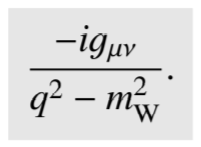
\includegraphics[width=11cm]{NuclearPhysics/modules/weak-force/pics/w-propigator.PNG}
            \caption{Caption}
            \end{figure}
            
            
            The relation between Fermi Theory and modern electroweak theory is:
            
            \begin{equation}
                \frac{G_F}{\sqrt{2}} = \frac{g_w^2}{8m_w^2}
            \end{equation}
            
            
            The strength of the weak interaction is determined from low energy measurments, in particular the muon lifetime:
            
            \begin{equation}
                \Gamma(\mu^- \longrightarrow e^- \nu_{\mu} \Bar{\nu}_e) = \frac{1}{\tau_{\mu}} = \frac{G_F^2 m_{\mu}^5}{192 \pi^3}
            \end{equation}
            
            Which gives a Fermi constant of \myquantities{$G_F = 1.2 x 10^{-5} GeV^{-2}$}
            
            The dimensionless coupling constant of the weak interaction is $\alpha_W$ = 1/30, which is stronger than QED, but since the W is so massive it is much weaker at low energy. Since QED goes as 1/$q^2$ and weak goes as 1/($q^2-m_w^2$) = 1/$m^2$ at low energy, the ratio of weak interaction rates to QED rates is $q^4/m_W^4$ (since the matrix element is squared). 
            
    \section{Weinberg Angle}
        Charlie Prescott, measurement of sin2 theta w (How do you measure Weinberg angle and what does it mean?)
        
        
    \section{Weak Charge}
         Weak charge of the proton?
         QWEAK
        
    \section{Other}
        Need to understand energies of nuclear fission, nuclear beta decay (i.e. nuclear fission ~ 200 MeV, beta decay ~ 2 MeV)
        Weak hypercharge, weak isospin and strong hypercharge?
        Crossband transition? 
        nilson asymptotic quantum numbers
       
            
    \section{Neutrinos and Neutrino Oscillations}
        Solar neutrinos flux problem
            Homestake mine experiment, 600 tons of cleaning fluid (C2Cl4), reaction is:\\
            \begin{equation}
                \nu_e + ^37_17Cl \longrightarrow ^37_18Ar + e^- 
            \end{equation}
            
            Theorized to observe 1.5 interactions per day, but only saw 0.5 interactions per day. 
            SNO and Super K investigated further, development of PMNS matrix, neutrino mass hierarchy, development of short baseline, long baseline experiments.
            
            
    \section{CP violation and weak hadronic interactions}
            no antimatter regions of space due to lack of anniliation photons
            weak eigenstates of quarks differ from mass eighenstates, this gives us the CKM matrix
            The GIM mechanism explians the branching ratio discrepancy in KL
            Wolfenstein parameterization and complex phase
            Neutral kaon system, lightest strange hadrons so must decay weakly
            Kaon explaination
            Strangeness oscillations, mass difference on order of $10^-15$ GeV. 
            
            \begin{figure}[H]
                \centering
                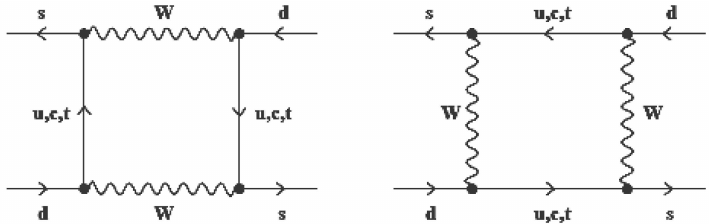
\includegraphics[width=11cm]{NuclearPhysics/modules/weak-force/pics/kaon-mixing-box-diagram.png}
            \caption{Caption}
            \end{figure}
            
            
            B mesons also oscillate and violate CP (I think)
            
            
    \section{Lepton universality}
        \indent In principle, the weak interaction could couple with different strengths to the different lepton generations. Experimentally, it is observed that all leptons couple with the same strength to the weak force, this is known as lepton universality. This is determined experimentally by measuring lepton decay rates, e.g.  
        
            \begin{figure}[H]
                \centering
                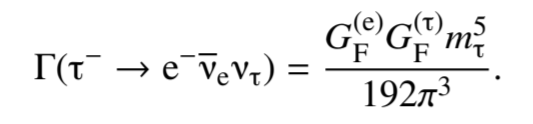
\includegraphics[width=11cm]{NuclearPhysics/modules/weak-force/pics/tau-decay-1.PNG}
            \caption{Caption}
            \end{figure}
            
            
            \begin{figure}[H]
                \centering
                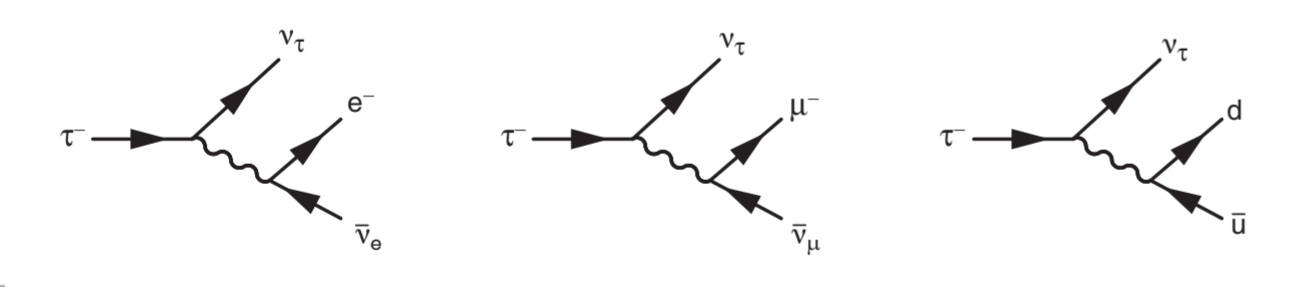
\includegraphics[width=11cm]{NuclearPhysics/modules/weak-force/pics/tau-decay-2.PNG}
            \caption{Caption}
            \end{figure}
            
    
    \section{Neutrino scattering}
        \subsection{Making a neutrino beam}
        
            \begin{figure}[H]
                \centering
                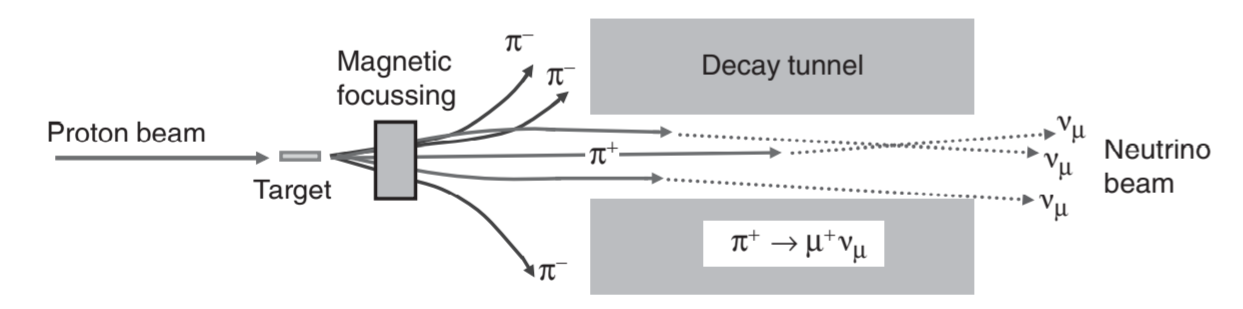
\includegraphics[width=11cm]{NuclearPhysics/modules/weak-force/pics/neutrino-beam.PNG}
            \caption{Caption}
            \end{figure}
            
        
        The canonical way to create a neutrino beam is to shoot a beam of protons at a target, producing charged pions, which are focused witha magnet to choose a particular charge / energy. The pions decay in flight over a few hundred meters. The muons from the charged pion decays are stopped in rock at the end of the tunnel before they decay so that no electron neutrinos are produced. 
        
        For neutrino DIS, there is a difference between neutrino-quark scattering, and anti-neutrino quark scattering. In order to conserve electric charge, the antineutrino can interact with an up quark, but not a down quark. 
        
        At low Q2, quasi-elastic scattering dominates, ($\nu_{\mu}n \longrightarrow \mu^- p$). Once we get to a few GeV, resonant inelastic processes, such as $\nu_{\mu}n \longrightarrow \mu^- \Delta^+ \longrightarrow \mu^- p \pi^0$ dominates, and further raising the energy we have neutrino DIS, where we blow up the nucleon.
        
        Considering the charged current interaction of muon neutrinos in DIS, we only have $\nu_{\mu}d \longrightarrow \mu^- u$, while for the antineutrino we only have 
        $\Bar{\nu}_{\mu}u \longrightarrow \mu^+ d$. The cross section for neutrino quark scattering is given cleanly as:
        
            \begin{figure}[H]
                \centering
                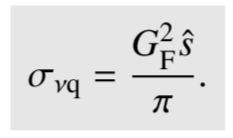
\includegraphics[width=11cm]{NuclearPhysics/modules/weak-force/pics/neutrino-quark-DIS.PNG}
            \caption{Caption}
            \end{figure}
            
        
        
        
        \myquantities{The cross section for antineutrino-quark scattering is 1/3 that of neutrino-quark scattering}. This difference is due to the fact that the weak charged current interaction only interacts with LH particles and RH antiparticles, and the factor of 1/3 pops out of the math. See Thomson 12.2 for the calculation details.  
        
        
        \section{Neutrino scattering experiments}
            THe CDHS experiment at CERN took data from 1976-84 with 30 - 200 GeV muon (anti) neutrino beam made from a 400 GeV proton source beam. It interacted with a 1K ton detector which had magnetised iron modules with wire drift chambers interspersed to detect muons. 
            
            Neutrino DIS is useful as it provides a direct measure of the antiquark content of the nucleon. 
            
            $F_3$ provides a direct measurement of the sum of the PDFs for the valence quarks alone. If there are three valence quarks in the nucleon, then we  have the Gross-Llewellyn-Smith sum rule:
            
            \begin{figure}[H]
                \centering
                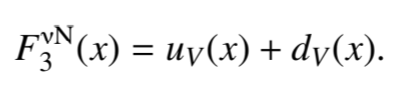
\includegraphics[width=11cm]{NuclearPhysics/modules/weak-force/pics/f3-nuN.PNG}
            \caption{Caption}
            \end{figure}
            
            
                \subsection{Gross-Llewellyn-Smith Sum Rule}
        If there are three valence quarks within the nucleon, then the below equality will hold:\\
        $\int_{0}^{1} F_3^{\nu N}(x)dx = \int_{0}^{1}u_v(x) + d_v(x) dx = 3 $\\
        The measurement of $xF_3^{\nu N}(x)$ is consistent with this prediction. 
        
        Charged current ep scattering was also studied at HERA at high energies, which was identified by missing momentum imbalance in the plane transverse to the beam axis. 

    
        Ratio of neutrino to antineutrino scattering scross sections off of an isoscalar target:
        
            \begin{figure}[H]
                \centering
                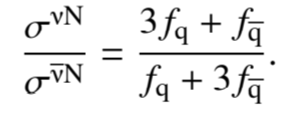
\includegraphics[width=11cm]{NuclearPhysics/modules/weak-force/pics/isoscalar-neutrino.PNG}
            \caption{Caption}
            \end{figure}
            
        
        Here, $f_q$ and $f_{\Bar{q}}$ are the fractions of the nucleon meomentum respectively carrid by quarks and the antiquarks:
        
            \begin{figure}[H]
                \centering
                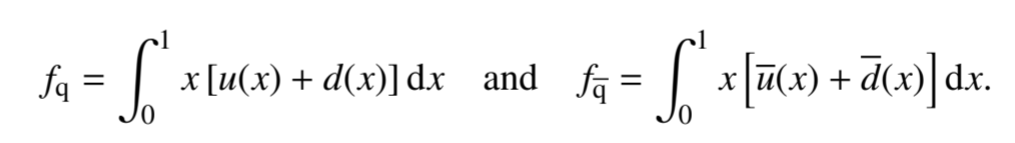
\includegraphics[width=11cm]{NuclearPhysics/modules/weak-force/pics/fqfbarq.PNG}
            \caption{Caption}
            \end{figure}
            
        
        This ratio was measured by CDHS and came out to a value of 2. If there were no aniquarks in the nucleon $f_{\Bar{q}}$ would equal 0, and the ratio would equal 3. However, the value being 2 corresponds to $f_{\Bar{q}}$ = 0.1 and $f_q$ = 0.4. This means only about half the momentum of the proton is carried by quarks and antiquarks, with the other 50\% being carried by gluons. 
        
        
        We need to add a F3 structure function to account for parity violation in weak interactions to scattering cross sections:
        
        
            \begin{figure}[H]
                \centering
                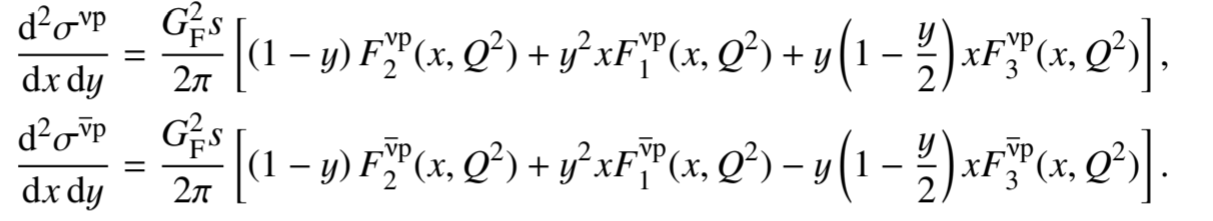
\includegraphics[width=11cm]{NuclearPhysics/modules/weak-force/pics/neutrino-f1f2f3.PNG}
            \caption{Caption}
            \end{figure}
            
        
        NuTeV in Fermilab measured these cross sections to map out the structure functions, and using parton model predictions
        
            \begin{figure}[H]
                \centering
                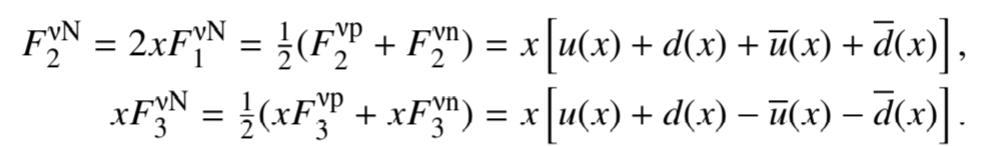
\includegraphics[width=11cm]{NuclearPhysics/modules/weak-force/pics/parton-predictions.PNG}
            \caption{Caption}
            \end{figure}
            
        
        We can take the difference of F2 and F3 as a direct measure of the antiquark content of the nucleon - we see the x distribution of antiquarks is largest at low values of x, as expected. 
        
        
        
            \begin{figure}[H]
                \centering
                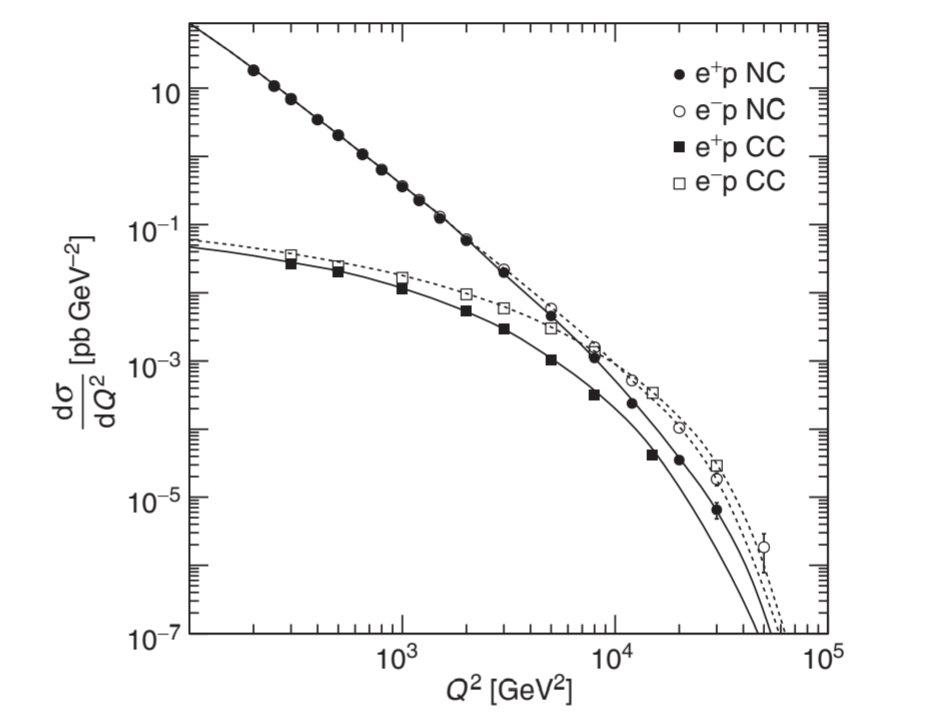
\includegraphics[width=11cm]{NuclearPhysics/modules/weak-force/pics/electroweak-scattering.PNG}
            \caption{Caption}
            \end{figure}
            
        
        Once we get to high Q2, the NC cross section includes signifcant contributions from both photn and Z exchange diagrams.
        
        
        
        
        \section{Neutrinos}
            How do we know neutrinos have distinct flavors?
                - neutrinos produced from beta decay always was observed to produced electrons in subsequent interactions, muon neutrinos were always observed to produced muons in subsequent interactions. 
                
            \begin{figure}[H]
                \centering
                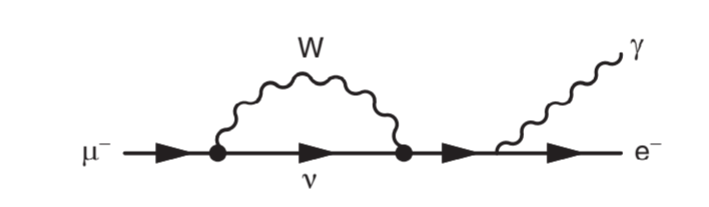
\includegraphics[width=11cm]{NuclearPhysics/modules/weak-force/pics/neutrino-distinction-diagram.PNG}
            \caption{Caption}
            \end{figure}
            
                
                Also, muons could change into electrons if neutrinos were not distinct, but htis is not observed either. 
                
            Neutrino flux from the sun - $1x10^38$ per second. 
            
            \begin{figure}[H]
                \centering
                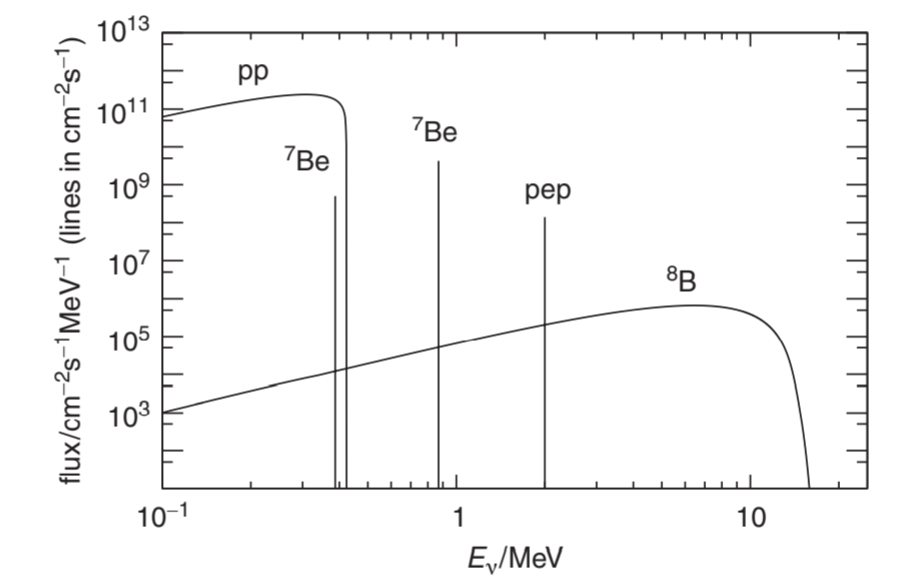
\includegraphics[width=11cm]{NuclearPhysics/modules/weak-force/pics/solar-neutrino-flux.PNG}
            \caption{Caption}
            \end{figure}
            
            
            Homestake mine experiment - was sensitive to the High energy Boron 8 neutrinos. SAGE and GALLEX, using gallium as a target, was sensitive to low energy neutrinos from the pp chain. Also observed a defiicit. 
            
            SuperK and SNO sorted out the problem by observing all (or many) neutrino decay pathways, which then made sense, in light of neutrino oscillations
            
            \begin{figure}[H]
                \centering
                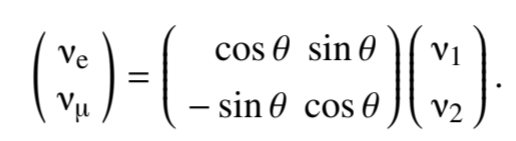
\includegraphics[width=11cm]{NuclearPhysics/modules/weak-force/pics/2-flavors.PNG}
            \caption{Caption}
            \end{figure}
            
            
            \begin{figure}[H]
                \centering
                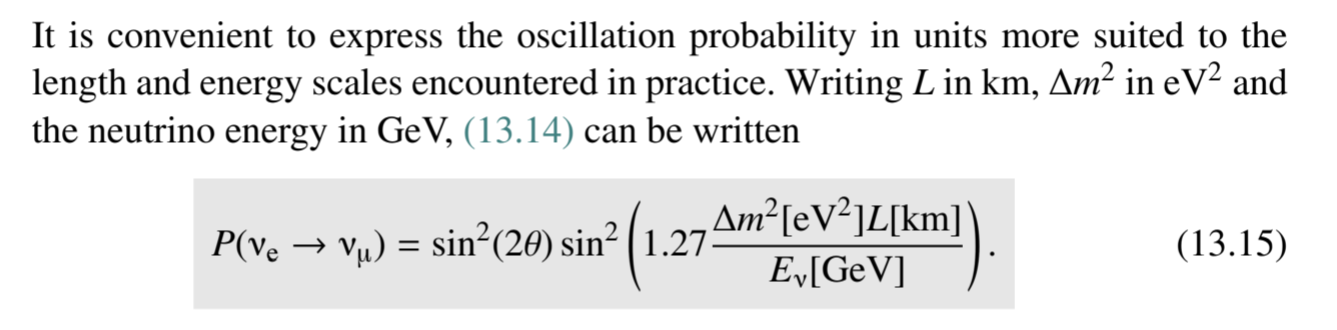
\includegraphics[width=11cm]{NuclearPhysics/modules/weak-force/pics/osc-prob.PNG}
            \caption{Caption}
            \end{figure}
            
            
            
            PMNS matrix:
            
            \begin{figure}[H]
                \centering
                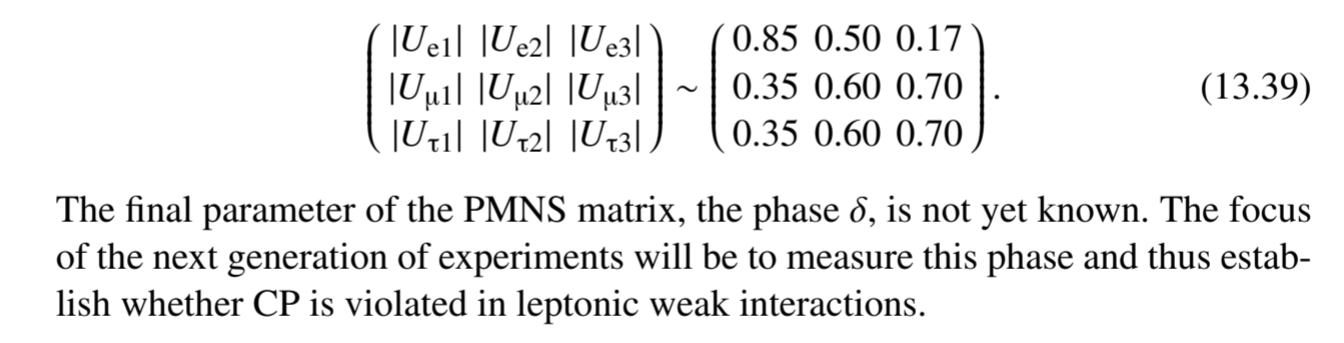
\includegraphics[width=11cm]{NuclearPhysics/modules/weak-force/pics/pmns.PNG}
            \caption{Caption}
            \end{figure}
            
            
            
        Z boson needed otherwise e+e- to WW cross section violates univatiry, neutral current discovered at Gargamelle, W and Z discovered at SPS.
        
        The weak boson decays proportional to 1 for charged lepton - neutrino pairs, and (color factor)x(CKM matrix element squared), e.g. udbar BR is proportional to 3*$V_{UD}^2$.
        
        The Z is a little bit more complicated. Since the Z is a mixture of pre symmetry breaking W0 and B0 bosons, each vertext factor has a factor of ($T_3 - qsin2\theta_W$, where T3 is the third component of weak isospin, and Q is the electric charge. Beceasue weak isospin is different for fermions of different chirality, the coupling is different as well.
        
        Since neutrinos have no charge, they just have T=1/2 for LH and T3=0 for RH. The charged leptons lose 0.23 for the weinberg mixing angle for the LH states, and gain it for the RH states. This is why neutrinos have a relative effective ratio of $1/2^2 = 1/4$, while charged leptons have a factor of $(1/2 - 0.23)^2 + 0.23^2 \approx 1/4^2 + 1/4^2 = 1/8$, which is why neutrinos have a BR of 20\% and charged leptons are only 10\%. 
        
        
        
        \section{Weinberg Angle}
            AKA weak mixing angle, parameter in electroweak theory, describing how much spontaneous symmetry breaking rotates the original $W^0$ and $B^0$ vector boson plane, producing the Z boson and the photon. 
            
            \begin{figure}[H]
                \centering
                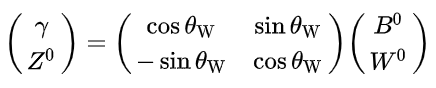
\includegraphics[width=11cm]{NuclearPhysics/modules/weak-force/pics/weinberg.PNG}
            \caption{Caption}
            \end{figure}
            
            
            It gives the relationship between the masses of the W and Z as:
            
            \begin{equation}
                m_Z = \frac{m_W}{\cos\theta_W}
            \end{equation}
            
            The wienberg angle also runs as a function of Q, and is measured at the Z scale most precisely, of 0.23. 
        
        
        
        \section{Example of QED and QCD Parity Invariance}
            \begin{equation}
                L = 1/4 F^{\mu \nu} F_{\mu \nu} = 1/4 \left( \partial_{\mu} A^{\nu} - \partial^{\nu} A_{\mu} \right)
            \end{equation}
            
            Now a parity transform yields $A^{\nu} \longrightarrow -A^{\nu}$, which then yields:
            
            \begin{equation}
                L = 1/4 \left( -\partial_{\mu} A^{\nu} + \partial^{\nu} A_{\mu} \right) = 1/4 \left( \partial_{\mu} A^{\nu} - \partial^{\nu} A_{\mu} \right)
            \end{equation}
            
            
            
            \section{Q-WEAK}
                JLab Hall C is home to the Q-Weak experiment - measuing weak charge of the proton. Parity violating electron scattering on the proton at low q2 - 0.025. Qweak = 1-4sin2theta2. I think they basically do this by making an assymmetr measuremnt to determine the extent of parity violation. This is important as it tests the running of the weinberg angle from the z pole down instead to very low Q2. 
                
                Experiment setup:
                scatter longitudinally polarized electrons from liquid hydrogen
                flip the electron spin and see how much the scattered fraction changes
                the difference is proportional to the weak charge of the proton.
                
                up weak charge: 1 - 8/3 sin2wienberg approx 1/3
                down quark -1 + 4/3 sin2weinberg approx -2/3
                thus neutron weak about -1, proton weak about 0.08
                
                
                \begin{figure}[H]
                    \centering
                    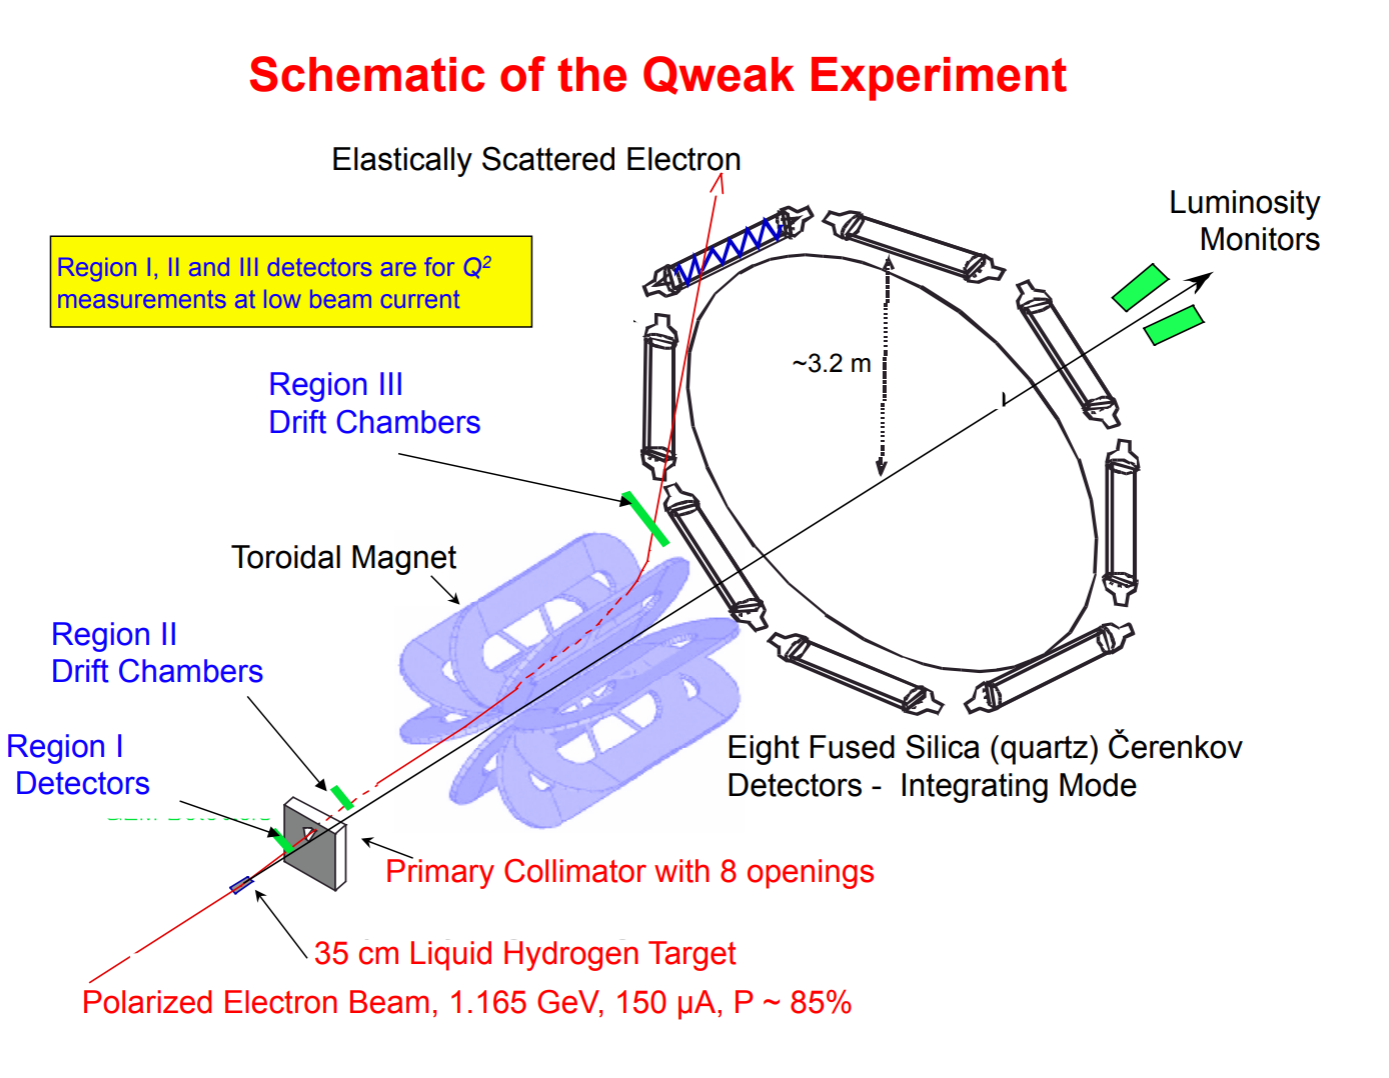
\includegraphics[width=11cm]{NuclearPhysics/modules/weak-force/pics/qweak.png}
                \caption{Caption}
                \end{figure}
                
                
            
            \section{PREx and CRex}
                Lead-208 (Pb) Radius Experiement in Hall-A, uses the parity violating weak neutral interaction to probe the neutron distribution in a heavy nucleus, specifically lead 208, thus measuring the RMS neutron radius to 1\% accuracy. Its sister experiment is CREX (same idea but with calcium 48). The idea is since the neutron has a weak charge of -1, and the proton has a weak charge of almost zero (0.08) by measuring the weak neutral current asymmetry, you are basically just measuring the neutron.  I think the idea is to measure the weak form factor and extract the radius by a kind of generalized rosenbluth separation, but more details are \href{https://hallaweb.jlab.org/parity/prex/}{here} and \href{https://hallaweb.jlab.org/parity/prex/prexI_prc.pdf}{here}.
                